\section{ByteNet}

The ByteNet model is an alternative approach to neural machine translation, it specifically focuses on having linear computational complexity, having a resolution preserving encoding, and be a charecter-level translation model \cite{bytenet}. This is somewhat diffrent from existing popular models such as the Sutskever 2014 model \cite{sutskever-2014-nmt} and the attention based Bahdanau 2015 model \cite{bahdanau-2015-nmt}.

Note that the model presented here is a simplified version of the original ByteNet model \cite{bytenet}. First, there are no bags of characters, only individual characters are used as the sentence representation. Secondly, the Sub-Batch normalization in the decoder is replaced by Layer Normalization, besides being a simpler solution than Sub-Batch Normalization this could also improve the model performance \cite{layer-normalization}.

\subsection{Word-Based Neural Machine Translation Models}

To understand the pros of ByteNet and how it differs from existing word-based model, a short introduction to two popular word based models, Sutskever 2014 \cite{sutskever-2014-nmt}, and Bahdanau 2015 \cite{bahdanau-2015-nmt}, is given. Later in the ByteNet chapter the corns will be discussed. 

\subsubsection{Sutskever Model}

\begin{equationbox}[H]
\begin{equation*}
\begin{aligned}
\text{encoding:} & \\
& \mathbf{h}_j = f(\mathbf{x}_j, \mathbf{h}_{j-1}) \quad \forall j \in [1, |S|] \\
\text{decoder:} & \\
&\mathbf{s}_i = \mathrm{g}(\mathbf{h}_{|S|}, \mathbf{s}_{i-1}) \\
&\mathbf{y}_i = \mathrm{softmax}(\mathbf{s}_i) \quad \forall i \in [1, |T|] 
\end{aligned}
\end{equation*}
\caption{The Sutskever 2014 model \cite{sutskever-2014-nmt}.}
\end{equationbox}

The Sutskever 2014 model \cite{sutskever-2014-nmt} was one of the first neural machine translation models to shows state-of-the-art performance on the WMT 2014 dataset.

The general idea is to encode a sequences of words using a recurrent neural network, the last encoder state is then used to initialize the decoder. The decoder iterates using the previously predicted word. While this approach is mathmatically elegant, encoding the source sentense ($S$) into a finite sized vector $h_{|S|}$ is in practice very difficult. The original implementation required a 8000 real valued dimentional vector for the sentence encoding. They also limited the source vocabulary to 16000 words and 8000 words for the target vocabulary.

Word-based neural machine translation models have shown to work well in practise, however they also have obviouse limitations. Words not in the vocabulary can't be translated, a common issue is names which for charecter-based models are very easy to translate because they require no translation. The softmax of a large vocabulary is also expensive, in the original Sutskever implementation they used 4 GPUs for just the softmax and 4 more GPUs for the rest of the network. This again can be solved by using charecter-based models because the ``vocabulary'' is just the diffrent letters, which there are a lot fewer off.

Using charecter instead of words in the Sutskever model may seam like a good idea at first, however the source and target sequences becomes much longer. Long sequences are difficult to encode and decode because the state is updated in each iteration, thus the state produced for the begining of the sentence is easily forgotten. In theory LSTM units solves this vanshing-moment issue, but in practise it still exists. In particullar Sutskever reversed the input sentence to get better performance, if there where no memory issues reversing the input sentence should have no effect.

\subsubsection{Bahdanau Attention Model}

\begin{equationbox}[H]
\begin{equation*}
\begin{aligned}
\text{encoding:} & \\
& \mathbf{h}_j = f(\mathbf{x}_j, \mathbf{h}_{j-1}) \quad \forall j \in [1, |S|] \\
\text{attention:} & \\
& e_{ij} = a(\mathbf{s}_{i-1}, \mathbf{h}_j) \\
& \bm{\alpha}_i = \mathrm{sparsemax}(\mathbf{e}_i) \\
& \mathbf{c}_i = {\textstyle \sum_{t=1}^T} \alpha_{it} \mathbf{h}_t \\
\text{decoder:} & \\
&\mathbf{s}_i = \mathrm{g}(\mathbf{c}_i, \mathbf{s}_{i-1}) \\
&\mathbf{y}_i = \mathrm{softmax}(\mathbf{s}_i) \quad \forall i \in [1, |T|] 
\end{aligned}
\end{equation*}
\caption{The attention based Bahdanau 2015 model \cite{bahdanau-2015-nmt}.}
\end{equationbox}

Bahdanau et. al. solved this memory issue by letting the decoder look at selected parts of the encoding state sequence. It does this though what is called an attention mecanishim. The attention $\bm{\alpha}_i$ is a weight vector, that is used in a weighted mean calculation over the encoded states $\mathbf{h}_t$. The weights a calculated using a sub-network that depends on the previuse output state $\mathbf{s}_{i-1}$ and the encoding states. The weighted mean is then used to calculate the next output state $\mathbf{s}_{i}$.

The attention mecanishim essentially recalculate a new encoding vector for each output state. This creates what called a resolution preserving encoding, that is an encoding which size depends on the source sequence, this is diffrent from the Sutskever model that uses a fixed sized vector. The Bahdanau et. al model is words-based and achieved state-of-the-art like performance. On the surface there is nothing that prevents the Bahdanau et. al. model from being chatecter-based, but by looking at the computational complexity it becomes clear that using chatecters is not a viable solution.

In each iteration on the output sequence, the attention model needs to calculate the weighted mean over the encoding sequence, this takes $\mathcal{O}(|S|)$ time. These calculations can not be reused in the next iteration because they also depends on the output state from the previuse iteration $s_{i-1}$. The attention thus needs to be recaulated for each output state, resulting in a computational complexity of $\mathcal{O}(|S||T|)$.

Having this quadratic-like computational complexity $\mathcal{O}(|S||T|)$, means that using characters instead of words dramatically increases the running time.

\subsection{ByteNet Residual Block}

Before explaining the full ByteNet network, a central component of the ByteNet model called the \textit{ByteNet residual block} needs to be explained first. There are two variations of this an \textit{Encoder Residual Block}, and a \textit{Decoder Residual Block}. First the encoder version is explained and then some slight alterations of this will turn it into the decoder version. For a visual representation see Figure \ref{fig:bytenet:residual-block}.

\subsubsection{Encoder Residual Block}

\subsubsection{Decoder Residual Block}

\begin{figure}[h]
    \centering
    \begin{subfigure}[b]{0.45\textwidth}
        \centering
        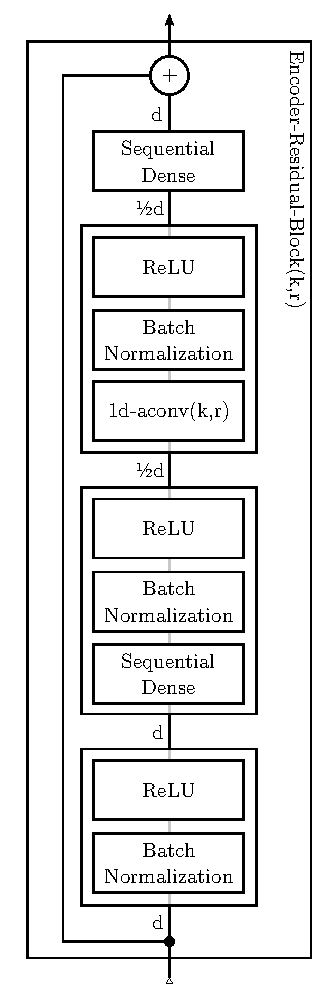
\includegraphics[scale=1]{theory/bytenet-residual-block.pdf}
        \caption{Residual Block used in encoder.}
    \end{subfigure}
    ~ %
    \begin{subfigure}[b]{0.45\textwidth}
        \centering
        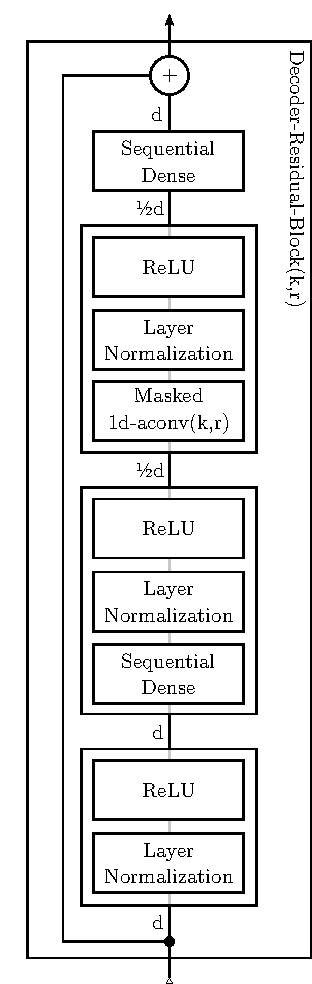
\includegraphics[scale=1]{theory/bytenet-residual-block-causal.pdf}
        \caption{Residual Block used in decoder.}
    \end{subfigure}
    \caption{The residual blocks used in the ByteNet model. The blocks are denoted by Encoder-Residual-Block$(k,r)$ and Decoder-Residual-Block$(k,r)$, where $k$ is the kernel width and $r$ is the dialation rate.}
    \label{fig:bytenet:residual-block}
\end{figure}


%* A simpler model, reducing computation and simplify implementation, there is also reason to belive that layer normalization will provide better results for the ByteNet model.

\FloatBarrier
\subsection{Encoder}
\subsection{Decoder}
\subsection{Forward Pass}
